\documentclass{article}
\usepackage{tikz}

\begin{document}

\begin{figure}[h]
    \centering
    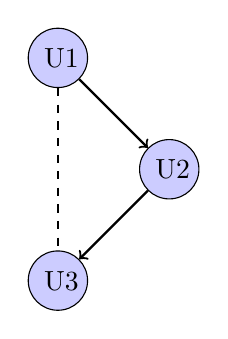
\begin{tikzpicture}[node distance=2cm,
                        every node/.style={circle, draw, fill=blue!20, text width=1em, align=center}]
        
        % Nodes
        \node (U1) {U1};
        \node (U2) [below right of=U1] {U2};
        \node (U3) [below left of=U2] {U3};
        
        % Edges
        \draw[->, thick] (U1) -- (U2);
        \draw[->, thick] (U2) -- (U3);
        
        % Additional edges to create a collider structure
        \draw[dashed, thick] (U1) -- (U3);
        
    \end{tikzpicture}
    \caption{Collider Causal Structure for Experiment 3}
    \label{fig:collider_structure}
\end{figure}

\end{document}